\documentclass{article}
\usepackage[utf8]{inputenc}
\usepackage[spanish]{babel}
\usepackage{graphicx}
\usepackage{subcaption}
\usepackage[toc]{appendix}
\usepackage{amsmath}
\usepackage{amssymb}
\graphicspath{ {./images/} }
\usepackage{biblatex} %Imports biblatex package
\addbibresource{name.bib} %Import the bibliography file
\usepackage{listings}
\usepackage{amssymb}

\decimalpoint

\usepackage{xcolor}

\definecolor{codegreen}{rgb}{0,0.6,0}
\definecolor{codegray}{rgb}{0.5,0.5,0.5}
\definecolor{codepurple}{rgb}{0.58,0,0.82}
\definecolor{backcolour}{rgb}{0.95,0.95,0.92}

\lstdefinestyle{mystyle}{
    backgroundcolor=\color{backcolour},   
    commentstyle=\color{codegreen},
    keywordstyle=\color{magenta},
    numberstyle=\tiny\color{codegray},
    stringstyle=\color{codepurple},
    basicstyle=\ttfamily\footnotesize,
    breakatwhitespace=false,         
    breaklines=true,                 
    captionpos=b,                    
    keepspaces=true,                 
    numbers=left,                    
    numbersep=5pt,                  
    showspaces=false,                
    showstringspaces=false,
    showtabs=false,   
    tabsize=2
}
\lstset{style=mystyle}


\title{Una Revisi\'on de M\'etodos de Evaluaci\'on Econ\'omica en Salud }
\author{Joaquín Viola-Chiazzaro \& Ramón Álvarez-Vaz }
\date{Julio de 2023}

\begin{document}

\begin{titlepage}
    \begin{center}
        \vspace*{3cm}
            
        \Huge
        \textbf{Evaluación Economica de Tratamientos Médicos-(Una Revisi\'on de M\'etodos de Evaluaci\'on Econ\'omica en Salud)}
            
        \vspace{1cm}
        \huge
        Instituto de Estadística - FCEA

        \vspace{1.5cm}
        \Large
            
        \textbf{Joaquín Viola-Chiazzaro \& Ramón Álvarez-Vaz}

        \vfill
        
            
        \vspace{1cm}
            
        
\includegraphics[width=1\textwidth]{logoFCEA.png}
        \\
        
        \Large
        
    \end{center}
\end{titlepage}

\maketitle
\tableofcontents
\newpage

\section{Resúmen}

En este trabajo se pretende hacer un repaso sobre distintos métodos de evaluación económica en la salud, viendo el análisis costo-beneficio y costo-utilidad pero prestando especial interés en el análisis costo-efectividad.
También se hará una breve introducción sobre los distintos aspecto a tener en cuenta a la hora de hacer una evaluación económica, cómo la obtención de los datos sobre los costos de los tratamientos, así como de las medidas de efectividad y su obtención.
Se introducirá el concepto del ratio incremental de costo-efectividad y el incremento del beneficio neto cómo herramientas para la toma de decisiones.
Se presentarán métodos frecuentistas de intervalos de confianza y métodos de bootstrap para las estimaciones de los parámetros de costos y de efectividad.
Por último se hará una breve presentación de los métodos bauesianos para la evaluación económica de tratamientos médicos.

\section{Introducción}

La evaluación económica en el ámbito de la salud es un área que ha tenido un constante desarrollo en las últimas décadas. Cómo en la mayoría de los problemas económicos, la evaluación económica de tratamientos médicos busca determinar la distribución óptima de los recursos (que son limitados), en las distintas demandas (que pueden ser ilimitadas).
\
En este documento trabajaremos con los casos en los que deseamos evaluar dos tratamientos médicos, que en general tienen distintos costos, y distintos resultados.
\
En la primera parte buscaremos brindar una aproximación a los métodos de evaluación económica más usados, prestando principal interés en la evaluación de costo-efectevidad. También en cómo obtenemos las resultados de costo y efectevidad para aplicar las técnicas de evaluación, y en la interpretación de los resultados

\

En una segunda instancia, buscaremos implementar métodos Bayesianos para el análisis de costo-efectevidad, se seguirán resultados del libro "Bayesian Methods in Health Economics" de Gianluca Baio, y se usarán datos y códigos de R planteados en "Bayesian Cost-Efectivenness Analysis with the R Package BCEA" del mismo autor.
 
\section{Evaluación Económica}

Los métodos de evaluación económica, surgen de resolver el problema económico de asignar recursos limitados, para maximizar los beneficios, es un conjunto de técnicas que pretenden medir los resultados de varias alternativas, y sirven de apoyo para la toma de decisiones. No buscan reducir los costos, si no guiar a los tomadores de decisiones en la mejor opción de gastar los recursos según los resultados obtenidos.

\

Usualmente se utilizan para comparar dos alternativas de inversión, por ejemplo en dos proyectos distintos, o para tomar la decisión de invertir en algo o no, cómo puede ser el arreglo de una máquina en una empresa de producción, o el cambio de una máquina por una más nueva.

\

Los métodos de evaluación económica no guiaran necesariamente las decisiones a aquella alternativa que sea más barata, si no que tendrá en cuenta los resultados que se obtienen, aún si estos no son en términos monetarios. Cómo puede ser el tiempo de viaje de los ciudadanos por la construcción de un puente, o los beneficios o contras para el medio ambiente por determinada obra.
Es así que en el control de los gastos públicos, se han utilizado estas herramientas en áreas cómo el transporte u otras obras públicas, pero recién en la década del 80’ ha tenido un auge en la
salud.

\subsection{Evaluación Económica En Salud}

En el sistema sanitario en general, nos encontramos ante el problema de tener recursos limitados, para atender necesidad ilimitadas, sumado a que los tratamientos tienen costos altos, por lo que motiva la necesidad de aplicar métodos de evaluación económica que comparen dos tratamientos frente a una enfermedad, para tomar la decisión de seguir con el actual, o cambiar a un nuevo tratamiento (Elías Moreno). A su vez, Weinsten y Stason (1977) plantean que la sociedad debe maximizar los beneficios agregados, esto motiva la necesidad de aplicar una metodología que una los costos de los tratamientos, junto a los resultado de los mismos ( qué no están medidos en términos monetarios)

\

Desde la década del 1970, ha habido un aumento en la demanda de la atención médica, lo que ha generado un aumento en la cantidad de intervenciones disponibles, esto ha llevado a que los tomares de decisiones en cuanto a los gastos médicos, necesiten estar más informado sobre los resultados y los costos para poder tomar mejores decisiones, algunos de los factores principales que ha llevado a la necesidad de comparar costos y beneficios en el sistema sanitario son: el aumento de la población mayor, consecuencia de un aumento en la esperanza de vida, el aumento de la presencia de patologías crónicas y degenerativas, la mejora en las técnicas de diagnósticos, las innovaciones tecnológicas que generan mejores resultados en salud, pero tienen mayores costos. (Gianluca Baio) (Soto Álvarez)

\

Cómo un ejemplo del aumento del gasto en salud, en Estados Unidos, en 1972, el gasto en salud era de U\$S400 pér capita, y en 2011 había ascendido a más de U\$S8000, pasando de un 7\% del PBI, a un 17\%.
En el mismo período, en UK, el porcentaje del PBI destinado a salud pasó de un 4,6\% a 9,4\%, en Francia de 6,2\% a 11,6\%, en Alemania de de 7,3\% a 11,3\% y en Japón de 4,8\% a 10\% (Glick, 2011), es por esto que los distintos países han buscado distintos métodos para controlar los gastos en salud. Que podemos diferenciarlos en métodos a nivel Macro, y a nivel Micro, estos últimos son en los que nos centraremos a lo largo de este documento.

\

Existen agencias a nivel nacional e internacional que hacen estos análisis para poder brindar mayor información a quienes toman las decisiones a nivel gubernamental. (Zárate, 2010) Por otro lado se observa, que a mayor progreso médico alcanzado, tenemos un mayor costo para obtener aún mejores resultados. (Sacristan, 2004)

\

El primer país en hacer obligatorios los análisis costo-efectividad para la financiación de medicamentos y tecnologías fue Australia en 1994, y de a poco algunos países cómo Canadá u otros de la Unión Europea lo han ido implementando, tanto cómo requisito, pero algunos cómo recomendación. Esto ha motivado que se haya extendido el desarrollo de herramientas para medir la efectividad y los resultados tanto a nivel paciente cómo a nivel social, así cómo también la posibilidad de extrapolar resultados de un país a la población a otro, sin perder rigurosidad científica (Soto Álvarez)

\

El desarrollo de esta área y ha generado el interés de numerosos investigadores que han ondeado en las técnicas y las metodologías para la toma de decisiones. Esto ha generado un crecimiento exponencial de artículos sobre análisis económico en salud en las últimas décadas.

\

Nota: en el desarrollo del documento se hablará indistintamente de medicación, tratamiento y tecnología, salvo que se indique lo contrario.

\subsection{Los Distintos Métodos}

Existen distintos métodos para la comparación de tecnologías, basados en los resultados y los costos de las mismas.
\
Por lo general buscaremos comparar tratamientos alternativos, contra el tratamiento actual, o status quo, en algunos casos más avanzados se compararan más de dos alternativas.

\

Estos métodos se diferencian principalmente en la forma de medir los resultados, y nosotros los separaremos en los 3 principales: costos-beneficios, costos-utilidad y costo-efectividad. Este último será el que nos resultará de principal interés.

\subsubsection{Análisis Costos-Beneficios}

Para el análisis costos-beneficios es necesario tener los costos y efectos medidos en la misma escala, usualmente en términos monetarios.
En estos casos nuestro criterio de selección es que $Beneficio > Costo$, y en particular maximizaremos $Beneficio-Costo$.

\

Resulta bastante inmediata la relación de este análisis con la teoría económica del bienestar, dónde el bienestar social es la suma de los bienestares individuales, evaluaremos mejoras en el bienestar social neto en la aplicación de los tratamientos. Es por esto que debemos lograr expresear todos los costos, beneficios y prejuicios para la salud en térmios monetarios
\
Su principal ventaja es poder medir tratamientos que tienen distinta medida de efectividad, pero resulta difícil transformar las "unidades de salud" en unidades monetarios.

\subsubsection{Análisis Costo-Efectividad}

En esta técnica, comparamos los tratamientos en términos de efectividad, cómo puede ser años de vida ganado, mejoras en el estado de salud, presión sanguínea o nivel de colesterol (sobre estas formas de medir la efectevidad se profundizará en la siguiente sección).

\

En este caso el costo y la efectividad no estarán medidos en las mismas unidades. Por lo que los criterios de selección pasan a ser un poco ambiguos. Resulta obvio que si a menor costo en el tratamiento alternativo, obtenemos mayor efectividad, optaremos por cambiar de tratamiento, pero la duda surge cuando tanto los costos cómo la efectividad aumentan. Para estos casos se debe fijar un monto fijo, de disposición a pagar para aumentar la efectividad en una unidad.

A cerca de este método profundizaremos más adelante, ya que es el más utilizado.

\subsubsection{Análisis Costos-Utilidad}

Se usa para casos especiales del análisis costos-efectividad, particularmente cuando la efectividad está medida en \textit{QALY's} (Quality-Adjusted Life Years), años de vida ajustado por la calidad.
\textit{QALY} es una medida compuesta de los efectos, integrada por las dos dimensiones principales de la salud, la cantidad y la calidad. Puede interpretarse cómo años de vida saludables equivalentes al estado de salud real.

\subsection{Implementación del Análisis Costo-Efectevidad}

A modo de comentario, empezaremos por aclarar las diferencias entre los conceptos de eficincia, eficacia y efectevidad.

La eficacia, es una medida de si un tratamiento cumple sus objetivos o no, la efectividad, involucra además la optimización de los recursos, mientras que la eficiencia es un concpeto económico que relaciona estos dos términos.

\

Como se comentó anteriormente, la evaluación económica mediante el análisis de costo efectevidad busca comparar simultaneamente los costo (medidos en términos económicos) y la efectevidad de los tratamientos (medidos justamente, en términos de efectevidad).

La herramienta que se implementará a lo largo de esta sección es el \textit{Ratio Incremental de Costo-Efectividad}, (\textbf{ICER}) por sus siglas en inglés, que medirá la variación de los costos según la variación en la efectevidad.

\subsubsection{Las variables del Análisis Costo-Efectevidad}

La primer variable de interés y en la que profundizaremos sobre la obtención de sus resultados es la \textbf{efectevidad}

La definiremos cómo la medida en la cuál un tratamiento cumple con los objetivos para los que fue diseñado bajo circunstancias óptimas.

Para poder medirla es necesario seleccionar las medidas que creemos relevantes para construir los índices de efectevidad

\

Para esto contamos con medidas de resultados finales y otras de resultados parciales. Algunas medidas de resultados finales son los años de vida ganado, o la probabilidad de una recaída, mientras que para las medidas de resultados parciales podemos tener la carga viral, la presión arterial o el colesterol, dependiendo del objetivo principal del tratamiento.
\

También se puede elegir más de una medida para medir la efectevidad, y hacer el análisis para cada una de las medidas, de forma de considerar la mayor cantidad de variables que pueden ser de interés.
Luego, si en el análisis de todas las medidas resulta mejor el mismo tratamiento, este será el tratamiento que debemos elegir, luego si hay medidas que dicen que es mejor un tratamiento y otras medidas que dicen que otro es el mejor, debemos elegir según la relevancia de cada medida.

\begin{center}
    \textbf{QALY's: una medida de la efectividad}
\end{center}

Muchas veces se utiliza cómo unidad de medida los años de vida ganados, o el aumento de la esperanza de vida ¿Pero qué pasa con la calidad de los años de vida?

\

Cómo ya se adelantó, \textit{QALY} pretende combinar los años de vida ganado y la calidad de estos años ganado según la intervención. Esto debido a que algunos tratamientos si bien cumplen con su objetivo, pueden ser invasibos y dañar la salud en otros aspectos.

Para construir las \textit{QALY's} es necesario poder medir la calidad de vida, medida en *HRQL* (Health-related quality life), cómo la calidad de los años ganados, asocidado a cada intervención. En general lo medimos entre 0 y 1, donde 1 es una calidad de vida óptima.
La combinación de los años de vida ganados y la calidad es lo que generan las \textit{QALY's}, debemos tener en cuenta que tienen cierta deficiencia para medir la salud mental o situaciones de cuidados paliativos.

\

Existen distintas herramientas que buscan agregar el efecto de la calidad de los años de vida ganado, muchas de estas son a modo de cuestionario a los pacientes que reciben los tratamientos.
Estos cuestionarios suelen incluir variables como el dolor, la autonomía, estado de ánimo, mobilidad y preguntas sobre las actividades usuales.

Uno de los cuestionaros más usados es el \textit{EuroQol 5D (EQ-5D)}, que en base a las respuetas de las distintas áreas presentadas anteriormente genera un índice mediante un algoritmo estandarizado para medir la calidad de vida.

\begin{center}
    \textbf{Fuentes de los datos de efectividad}
\end{center}

Esto no es un aspecto menor, ya que se debe incluir en los aspectos legales de un estudio, y es necesario especificar la fuente de los datos para que nuestros resultados sean válidos.
Por lo general se obtienen los datos de experimentos aleatorios bajo principios científicos.

Los pacientes son asingados aleatoriamente a uno de los tratamientos para minimizar el sesgo de los resultados.
En los ensayos clínicos solemos obtener mejores datos para hacer inferencia que en los estudios de observación.

\

Tenemos dos tipos de estudios distintos, que se pueden hacer al mismo tiempo, estudios de confirmación, que sirven para verificar la efectividad de un tratamiento, y estudios exploratorios, que buscan encontrar repuestas a distintos asuntos, pero no sobre la exactitud de los tratamientos.

Por otra parte, existen algunos puntos que debemos tener en cuenta a la hora de hacer un ensayo clínico. \textit{La selección de los pacientes}, estos son en general altamente definidos, y hace que no sea una muestra representativa de la población. \textit{La diferencia entre resultados en un ensayo y en la vida real}, debido a que los ensayos clínicos ocurren sobre condiciones ideales, que raramente se dan en la realidad. Por último, muchas veces tenenmos resultados intermedios porque tenemos un problema con el \textit{horizonte temporal} de nuestros ensayos.

\

Terminada la introducción sobre la obtención de los resultados de efectividad, haremos un breve repaso sobre la obtención de los \textbf{costos}, cómo obtenerlos y qué costos son relevantes para la evaluación económica en este caso.

\

Debemos identificar todos los costos que se hacen durante el ensayo clínico, y todos los recursos que son utilizados, expresados en términos monetarios. Haremos un breve repaso por los tipos de los costos, pero no nos centraremos en la construcción de la variable costo, en nuestros ejemplos vendrá dada.

\begin{itemize}
    \item \textbf{Costos Directos}: incluye todos los bienes y servicios usados durante el ensayo, el tiempo de los profesionales, los costos de los tratamientos.

    \item \textbf{Costos Indirectos}: También conocidos como costos de productividad, ya que están relacionados con los costos que tienen los pacientes por participar del ensayo clínico, cómo faltar al trabajo.

    \item \textbf{Costos Intangibles}: relacionados al dolor o sufrimiento que tienen los pacientes durante el ensayo.

    \item \textbf{Costos de Transición}: relacionado a los gastos de la investigación para la producción de nuevos tratamientos.
\end{itemize}

\subsection{Ratio Incremental de Costo-Efectevidad}

Cómo se mencionó anteriormente, el Ratio Incremental de Costo-Efectevidad (de adora en adelante \textit{ICER}) es una herramienta que sirve para medir el incremento de los costos, según el incremento en la efectividad, al comparar 2 tratamientos. Así que al comparar el tratamiento 1, supongamos tratamiento alternativo, contra el tratamiento 2, tratamiento de control, estaremos calculando $ICER_{1,2}$.

Sea $\gamma_i$ y $\epsilon_i$ el costo y la efectevidad asociados al tratamiento i, podemos ver el incremento del costo cómo $\Delta\gamma_{1,2}=\gamma_1-\gamma_2$ y el incremento de la efectividad $\Delta\epsilon=\epsilon_1-\epsilon_2$.

 \begin{equation}
    ICER_{1,2}= \frac{\Delta\gamma}{\Delta\epsilon} 
\end{equation}

Veamos que el $ICER_{1,2}$ es el aumento del costo por aumentar en una unidad la efectividad.

\

Cómo principalmente estaremos trabajando con muestras de la población objetivo, no podremos calcular el $ICER_{1,2}$, si no una estimación del mismo, que indicaremos $\widehat{ICER_{1,2}}$, y para su cálculo debemos hacer una estimación de los costos y la efectividad de los tratamientos, para lo que usaremos los costos y la efectividad promedio ($\bar{c}$ y $\bar{e}$) de cada uno de los tratamientos, así el cálculo de $\widehat{ICER_{1,2}}$ es:

\begin{equation}
    \widehat{ICER_{1,2}}= \frac{\bar{c_1}-\bar{c_2}}{\bar{e_1}-\bar{e_2}}
\end{equation}

Debemos observar que el valor del $\widehat{ICER_{1,2}}$ puede ser positivo o negativo según distintos factores, por lo que no podemos tomar cómo referencia un solo valor para decidir sobre los tratamientos, hay que poder interpretarlos bien.

\begin{equation}
    \widehat{ICER_{1,2}}
    \begin{cases}
        <0 & \bar{c_1} > \bar{c_2} \text{   y   }   \bar{e_1} < \bar{e_2} \\
        <0 & \bar{c_1} < \bar{c_2} \text{   y   }   \bar{e_1} > \bar{e_2} \\
        >0 & \bar{c_1} > \bar{c_2} \text{   y   }   \bar{e_1} > \bar{e_2} \\
        >0 & \bar{c_1} < \bar{c_2} \text{   y   }   \bar{e_1} < \bar{e_2} \\
    \end{cases}
\end{equation}

Vemos que cómo se decía anteriormente, el valor del ratio incremental puede ser negativo o positivo segúnd distintos factores. Por ejemplo, si los costos promedios del tratamiento 2 son más bajos que los del tratamiento 1, y la efectividad del tratamiento 2 es mayor que la efectividad del tratamiento 1, el $\widehat{ICER_{1,2}}$ será negativo, pero si los costos del tratamiento 2 son más altos que del tratamiento 1, y la efectividad del tratamiento 1 es mayor que la del tratamiento 2 también tendremos un valor negativo de $\widehat{ICER_{1,2}}$.

\

Es por esto, que al valor del $ICER_{1,2}$ lo acompañamos de una representación gráfica, para saber en qué situación nos encontramos, a esta representación la llamamos "Plano Costo-Efectividad" gráfico \ref{fig:1}.
\
En el eje horizontal de nuestro plano encontraremos $\Delta\epsilon$, el incremento de la efectividad, y en el eje vertical tendremos $\Delta\gamma$, el incremento de los costos. Además, veremos que el plano está dividido en dos partes, por una recta que pasa por el origen y tiene pendiente positiva \textbf{R}, esta recta nos divide el plano en las situaciones en las que eligiremos el tratamiento 2 y en las que eligiremos el tratamiento 1. Este valor de \textbf{R} representa la disponibilidad a pagar por una unidad extra de efectividad.
\
En nuestro plano, la zona coloreada en celeste, nos marca las situaciones en dónde eligiremos el tratamiento alternativo frente al tratamiento de control.
\
Se nota que en el cuadrante 4, sube la efectividad y baja el costo, por lo que el resultado es inmediato. Mientras que en los cuadrantes 1 y 3, debemos estar por debajo de la línea con pendiente \textbf{R}. Para el cuadrante 1, esto se cumple cuando $ICER_{1,2}<R$ mientras que en el cuadrante 3 cuando $ICER_{1,2}>R$. Por último, en el cuadrante 2 nunca optaremos por el tratamiento alternativo debido a que aumentan los costos y baja la efectividad.


\begin{figure}[htbp]
    \centering
    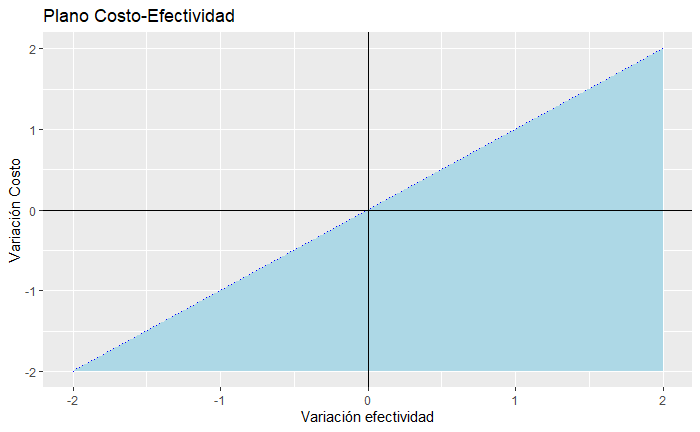
\includegraphics[width=1\textwidth]{grafi/Plano_Cost_Efect.jpg}
    \caption{Plano Costo-Efectividad}
    \label{fig:1}
\end{figure}
    

\subsubsection{Aplicación Análisis Costo-Efectevidad en dos tratamientos}

En esta sección usaremos un ejemplo del libro de Elías Moreno \textit{"Bayesian Cost-Effectiveness Analysis of Medical Treatments"}(tabla \ref{tabla:1}), en dónde tenemos los costos y la efectividad promedio de dos tratamientos.

\begin{table}[ht]
\centering
\begin{tabular}{lcc}
  \hline
 & Tratamiento 1 & Tratamiento 2 \\ 
  \hline
Costo Promedio & 7302.70 & 7142.28 \\ 
  Efectividad Promedio (QALY's) & 0.4024 & 0.3958 \\ 
 \hline
\end{tabular}
\caption{Ejemplo 1}
\label{tabla:1}
\end{table}

En donde obtenemos un incremento del costo de $\$160.42$ y un aumento de la efectividad de 0.0066 QALY'S al pasar del tratamiento 2 al tratamiento 1.
\
De esta forma $\widehat{ICER_{1,2}} = \$24306.06$ 

\

En este ejemplo, si la disposición a pagar es de \$20000 por una unidad extra de efectividad, no se estaría cambiando al tratamiento 1, pero para un R de \$25000 si.

\subsection{Incremento del Beneficio Neto}

El Incremento del Beneficio Neto (\textit{INB}) busca mejorar el \textit{ICER} en el sentido de que es más fácil de interpretar, con valores positivos ya podemos tomar una decisión. Pero para esto es necesario haber fijado el valor de \textbf{R} previamente.

\begin{equation}
    INB_{1,2} = R(\epsilon_1-\epsilon_2)-(\gamma_1-\gamma_1) = R\Delta\epsilon-\Delta\gamma
\end{equation}

El \textit{INB}  está expresado en términos monetarios, dado que \textbf{R} lo está, y multiplica la efectividad que no tiene ninguna unidad de medida particular. Si la diferencia en la efectividad de un tratamiento a otro, multiplicada por la voluntad a pagar por cada unidad de efectividad extra, supera la diferencia de los costos, se cambiará de tratamiento.

Al igual que en el \textit{ICER} podemos tener la estimación de \textit{INB} usando los costos y la efectividad promedio.

\begin{equation}
    \widehat{INB_{1,2}} = R(\bar{e_{1}}-\bar{e_{2}})-(\bar{c_{1}}-\bar{c_{2}})
\end{equation}

Vemos que ahora, el $\widehat{INB}$ es una combinación lineal de parámetros que podemos estimar, y no es una fracción como lo era el $\widehat{ICER}$, podemos calcular facilmente la esperanza y la varianza de $\widehat{INB}$.

\begin{equation}
    \mathbb{E}(\widehat{INB_{1,2}})=R(\epsilon_1-\epsilon_2)-(\gamma_1-\gamma_2)
\end{equation}

\begin{equation}
    \mathbb{V}(\widehat{INB_{1,2}})=\sum_{i=1}^2(R^2\sigma^2_{e_i}+\sigma^2_{c_i}-2R\rho_i\sigma_{c_i}\sigma_{e_i})/n_i
\end{equation}

En donde la $\mathbb{V}(\widehat{INB})$ se puede estimar con el estimador de la varianza ($\widehat{\mathbb{V}(\widehat{INB})}$) sustituyendo la varianzas ($\sigma$) por las varianzas muestrales $s$, y la correlación ($\rho$) por la correlación muestral $r$.

\

Luego podemos pasar a construir la curva de aceptación de costo-efectividad, la misma mide la probabilidad de que $INB_{1,2}$ sea positivo para distintos valores de R, esto es $P(\widehat{INB_{1,2}>0}$. Para valores de R bajos, cuando la disposición a pagar por una unidad más de efectividad es baja, la probabilidad de que $\widehat{INB_{1,2}}$ sea positivo es muy baja, y para valores altos de R, tiende a 1.

\begin{figure}[htbp]
    \centering
    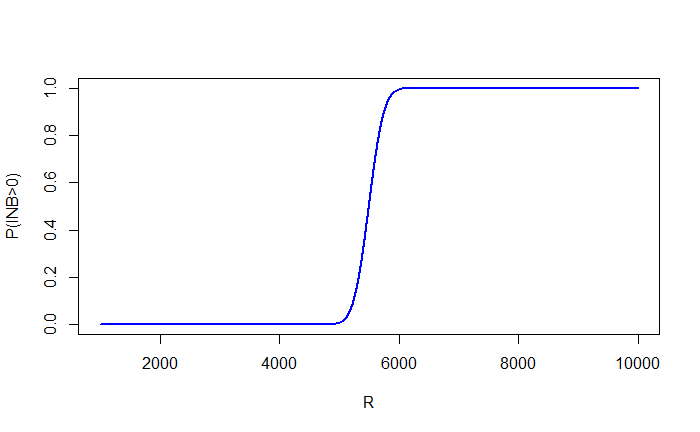
\includegraphics[width=1\textwidth]{grafi/Curva_acept.jpg}
    \caption{Curva de Aceptación}
    \label{fig:2}
\end{figure}

\subsection{Intervalos de Confianza}

Los resultados anteriores motivan la necesidad de obtener intervalos de confianza para los parámetros estimados, y así poder tener un intervalo de confianza para el \textit{INB}, que es lo que guiará las decisiones.

\

En esta sección abordaremos brevemente los métodos frecuentistas y de bootstrap para hacer intervalos de confianza de las estimaciones, más adelante se presentarán métodos bayesianos con el mismo fin, junto a los beneficios de estos.


\begin{center}
    \textbf{Aproximación Frecuentista}
\end{center}

Capitulo 2 de Elías Moreno.
Resulta claro que lo que estuvimos estimando hasta ahora, los costos y las medidas de efectividad de los tratamientos eran parámetros para poder construir el \textit{ICER} y el \textit{INB}. Hasta ahora se estuvieron tomando las medias muestrales cómo la representación de este parámetro, pero no teníamos herramientas para hacer los intervalos de confianza.
\
En esta sección, supondremos conocidas las distribuciones de los costos y efectividad, y con herramientas aprendidas en los cursos de inferencia estimaremos los parámetros de interés, y un intervalo de confianza para estos, dada la muestra.
La principal herramienta que utilizaremos es la función de verosimilitud, que está en función del parámetro que se desea estimar, y se toma como estimación del parámetro el valor para el cuál se maximiza la función de verosimilitud.

Teniendo la función conjunta de la muestra $f(x\mid \theta)$, cómo supondremos que las muestras son independientes, nuestra función conjunta será el producto de las funciones de cada individuo.

\begin{equation}
    f(x\mid \theta) = \prod_{i=1}^n f(x_i\mid \theta)
\end{equation}

Obteniendo también nuestra función de verosimilitud $\ell_x(\theta)$ que depende de $\theta$.

\begin{equation}
    \ell_x(\theta) = \prod_{i=1}^n f(x_i\mid \theta)
\end{equation}

Nuestro interés es encontrar el $\theta$ que maximice esa función, y ese será nuestra estimación puntual, cómo se mostrará a continuación, si estamos trabajando con una función conocida en que $\theta$ corresponde a la esperanza de la variable aleatoria, la estimación puntual corresponderá con la media de la muestra.

\textbf{Ejemplo: Distribución Normal}

Supongamos que los costos se distribuyen Normal, con media $\mu$ y varianza $\sigma^2$, esto es: $X \sim N(\mu,\sigma^2)$, la función de verosimilitud será:

\begin{equation}
    \ell_x(\mu,\sigma)= \sigma^{-n}exp\{-\frac{ns^2}{2\sigma^2}\}exp\{-\frac{n(\bar{x}-\mu)}{2\sigma^2}\}
\end{equation}

Con $\bar{x} = \sum_{i=1}^n x_i/n$ y $ns^2=\sum_{i=1}^n (x_i-\bar{x})^2$, donde $\bar{x}$ es el estimador de maxima verosimilitud de $\mu$ y $s^2$ el de $\sigma^2$.
\

Luego, como la variable aleatoria tiene distribución Normal, también lo tiene su media, entonces $\bar{x} \sim N(\mu,\sigma^2/n^2$, por lo que nos basta con determinar el nivel de confianza que deseamos en los parámetros para calcular un intervalo de confianza.

\

Si queremos trabajar con una confianza de un 95\% en la estimación de cada parámetro, esto es, un error máximo de un 5\% ($\alpha=0.05$), el intervalo de confianza del costo del tratamiento $i$ nos queda:

\begin{equation}
    IC_{(1-\alpha/2)100\%}(\gamma_i) = [\bar{c_i} - Z_{1-\alpha/2}\sigma_{\gamma_i}/\sqrt{n_i} , \bar{c_i} + Z_{1-\alpha/2}\sigma_{\gamma_i}/\sqrt{n_i}  ]
\end{equation}

Es un intervalo centrado en la estimación puntual $\bar{c_i}$, en donde $Z_{1-\alpha/2}$ es el valor para el cual una normal estandar (esperanza 0 y varianza 1) acumula $1-\alpha/2$ de probabilidad.

Luego, cambiando $\sigma_{\gamma_i}$ por $s_{c_i}$ obtenemos una estimación del intervalo de confianza.

\

Además, se puede aplicar el mismo resultado para la efectividad de los tratamientos, y obtener intervalos de confianza para $\epsilon_i$, y también se pueden utilizar distintas distribuciones en vez de la Normal obteniendo resultados parecidos.

\begin{center}
    \textbf{Método de Bootstrap No Paramétrico}
\end{center}

El bootstrap en general, toma a la muestra cómo la población, y re-muestra nuevamente, repitiendo el proceso muchas veces de forma computacional, para poder estimar una estimación del parámetro de interés, la varianza e intervalos de confianza.
Nosotros estaremos utilizando el bootstrap para estimar la variación de la efectividad y la variación de los costos, y sus respectivos intervalos de confianza.
Con estas estimaciones podremos graficar en el plano costo-efectividad tantos puntos cómo iteraciones hallamos hecho, representando estos puntos una pareja $(\Delta\epsilon,\Delta\gamma)$ de una iteración.

\

Briggs y William (2006) proponen que se hagan $B$ pasos, y en cada paso del bootstrap el tamaño de muestra de cada tratamiento sea igual a la cantidad de pacientes en cada tratamiento, pero al ser muestras con reemplazo, seguramente habrá muestras en que se repitan algún paciente y otro no salga.

Luego, para cada muestra tendremos ($\hat{\Delta_{ei}},\hat{\Delta_{ci}}$) y también tendremos $\widehat{ICER_{i}}$, y fijado un R podremos tener también $\widehat{INB_i}$ así cómo un estimador de la varianza y un intervalo de confianza.

\begin{figure}[htbp]
    \centering
    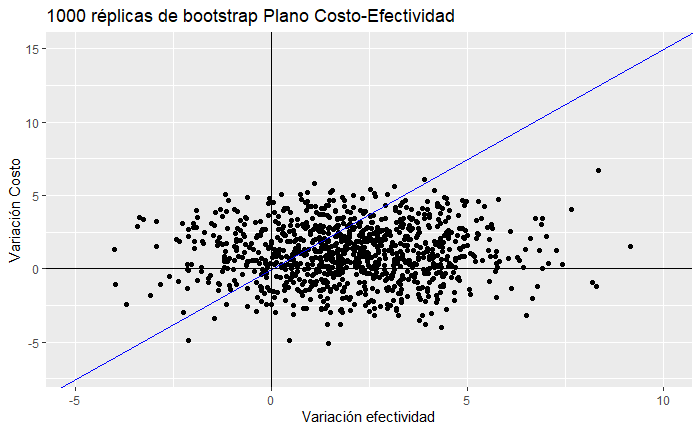
\includegraphics[width=1\textwidth]{grafi/boostrap.jpg}
    \caption{Representación de los ICER's para 1000 muestras obtenidas con bootstrap}
    \label{fig:3}
\end{figure}

El gráfico presentado en figura \ref{fig:3} no fue obtenido precisamente con el método de bootstrap, se hicieron mil simulaciones de dos normales, es meramente representativo.

\

Los intervalos de confianza basados en normalidad para el \textit{ICER} tienen serios problemas, ya que al ser un ratio, se vuelve muy inconsistente para valores de $\Delta_e$ muy cercanos a 0.

Se propone trabajar con intervalos de confianza construidos con el método de los percentiles, que además generan resultados consistentes para los tomadores de decisiones y replicables para el \textit{INB} y la curva de aceptación.



\section{Anexo}
\subsection{Código Gráficos}

Gráfico 1:
\begin{verbatim}
R=1
deltaeps <- seq(-2,2,by=0.01)
deltacost <- deltaeps*R
data <- as.data.frame(cbind(deltaeps,deltacost))
ggplot(data,aes(x=deltaeps,y=deltacost)) + geom_line(color="blue")+
  geom_ribbon(aes(ymin=-2,ymax=deltacost), fill="lightblue") +
  geom_hline(yintercept = 0, color = "black", linetype = "solid", size = 0.5) +
  geom_vline(xintercept = 0, color = "black", linetype = "solid", size = 0.5) +
  labs(title = "Plano Costo-Efectividad", x="Variación efectividad",y="Variación Costo")
\end{verbatim}


Gráfico 2:
\begin{verbatim}
R <- seq(1000,10000,by=1)
plot(R,pnorm(R,5500,200), type = "l",
     ylim = c(0, 1), ylab = "P(INB>0)", lwd = 2, col = "blue")
\end{verbatim}


Gráfico 3:
\begin{verbatim}
deltaefect <- rnorm(1000,mean=2,sd=2)
deltacosto <- rnorm(1000,mean=1,sd=2)
ICERS <- as.data.frame(cbind(deltaefect,deltacosto))

ggplot(ICERS, aes(x=deltaefect,deltacosto)) + geom_point() +
  geom_abline(intercept = 0,slope=1.5, color="blue") +
   geom_hline(yintercept = 0, color = "black", linetype = "solid", size = 0.5) +
  geom_vline(xintercept = 0, color = "black", linetype = "solid", size = 0.5) +
  labs(title = "1000 réplicas de bootstrap Plano Costo-Efectividad", x="Variación efectividad",y="Variación Costo") +
  xlim(-5,10) + ylim(-7,15)




\end{verbatim}

\section{Comentarios Personales}




\end{document}